\documentclass[dvipdfmx,12pt]{beamer}
\usepackage{bxdpx-beamer}
\usepackage{pxjahyper}
\usepackage{tikz}
\usepackage{here}
\usepackage{graphicx}
\renewcommand{\kanjifamilydefault}{\gtdefault}

\usepackage{amsmath}
\usepackage{amsfonts}
\usepackage{amssymb}
\usepackage{color}
\usepackage{tcolorbox}
\usepackage{forest}
\usepackage{ascmac}
\usepackage{fancybox}
\usetikzlibrary{arrows.meta}
\usetikzlibrary{positioning}

\usetheme{metropolis}  

% blockのスタイルをカスタマイズ
\setbeamercolor{block title}{bg=blue!30,fg=black} % タイトルの背景色とテキストの色
\setbeamercolor{block body}{bg=blue!10,fg=black} % ボディの背景色とテキストの色

\usepackage[usetype1]{uline--}

\title{第3回MPC勉強会}
\author{鶴原康太}

\begin{document}

    \frame{\maketitle}
    
    \begin{frame}{今回の目標}
        \footnotesize
      
        \begin{equation*}
            -\frac{\partial V}{\partial t}\left(x,t\right) = \min _u H\left(x, u, \left( \frac{\partial V}{\partial x} \right)^T\left(x, t\right), t \right)
        \end{equation*}
        \centering
        \begin{itemize}
            \item \colorbox{yellow}{前回のおさらい}
            \item 動的計画法
            \item HJB方程式
            \item 最小原理
            \item MPC導入
        \end{itemize}
    \end{frame}

    

    \begin{frame}{前回のおさらい}
        \scriptsize
        

        \begin{columns}
            \begin{column}{.4\textwidth}
                \begin{tcolorbox}[title=微分法]
                    \colorbox{yellow}{関数}の勾配を考える\\
                    停留するとある関数の最大or最小 \\
                    \colorbox{yellow}{点}の変動を考える\\
                \end{tcolorbox}
            \end{column}
            \begin{column}{.2\textwidth}
                \centering
                \tikz \draw[->](0,0) -- (1,0);
            \end{column}
            \begin{column}{.4\textwidth}
                \begin{tcolorbox}[title=変分法]
                    \colorbox{yellow}{汎関数(関数の関数)}の勾配を考える\\
                    停留するとある関数の全体を最大or最小\\ 
                    \colorbox{yellow}{関数}の変動を考える\\
                \end{tcolorbox}
            \end{column}
        \end{columns}

        微分法ではある曲線を最小化(最大化)することを考えていたけど、変分法ではある評価関数に基づいて関数全体を最小化(最大化)する関数を求める \\
        
        偏微分と似た考え方をする \\

        二点境界値問題の解 \\
        Euler-Lagrange方程式を満たす \\
        制約を含んだ場合 \\
    \end{frame}

    \begin{frame}{最適性条件まとめ}
        \fontsize{6.5pt}{6.5pt}\selectfont

        \begin{columns}
            \begin{column}{.5\textwidth}
                \begin{itembox}[l]{時間を考慮しない}
                    離散時間MPCでは予め時間を考慮して出した式から出た最適化問題を解いたから\\
                    最適化問題自体は時間を考慮しなくていい\\
                    Lagrangeの未定乗数法\\
                    \begin{align*}
                        L(x, \lambda) = f(x) + \lambda^T g(x)
                    \end{align*}
                    KKT条件\\
                    \begin{align*}
                        \nabla f(x^*) &+ \sum_{i=1}^m \lambda_i^* \nabla g_i(x^*) + \sum_{j=1}^n \mu_j^* \nabla h_j(x^*) = 0 \\
                        g_i(x^*) &\leq 0 \quad \text{for all } i \\
                        \lambda_i^* &\geq 0 \quad \text{for all } i \\
                        \lambda_i^* g_i(x^*) &= 0 \quad \text{for all } i \\
                        h_j(x^*) &= 0 \quad \text{for all } j
                    \end{align*}
                \end{itembox}
            \end{column}

            \begin{column}{.5\textwidth}
                \begin{itembox}[l]{時間を考慮}
                    Euler-Lagrange方程式\\
                    \begin{align*}
                        \frac{\partial L}{\partial x} - \frac{d}{dt} \left( \frac{\partial L}{\partial \dot{x}} \right) = 0
                    \end{align*}
                \end{itembox}
            \end{column}
        \end{columns}
    \end{frame}

    \begin{frame}{最適化の多様な定式}
        Q.なぜ似たようなものがいくつもあるのか??\\

        A.同時期(冷戦期)に2人の天才によって最適制御が定式化されたから\\

        \begin{columns}

            \begin{column}{0.5\textwidth}
                \centering
                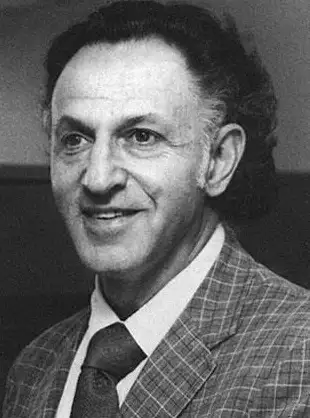
\includegraphics[clip, width = 2.0cm]{Bellman.png}\\
                {\tiny Bellman}
            \end{column}
        
            \begin{column}{0.5\textwidth}
                \centering
                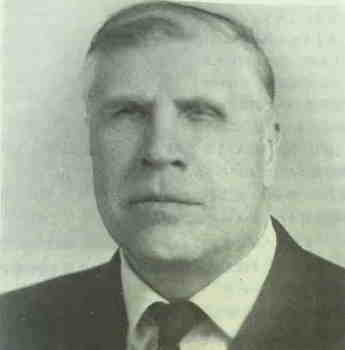
\includegraphics[clip, width = 2.0cm]{Pontryagin.png}\\
                {\tiny Pontryagin}
            \end{column}
        \end{columns}

        Bellmanによって動的計画法(Bellman方程式)\\

        Pontryaginによって最小原理(最大原理)\\

    \end{frame}

    \begin{frame}{動的計画法1}
        \footnotesize
        \begin{tcolorbox}[title=最適制御]
            \begin{align*}
                \dot{x}(t) &= f(x(t), u(t), t) \\
                J &= \psi(x(t_f)) + \int_{t_0}^{t_f} L(x(t), u(t), t) \, dt
            \end{align*}
        \end{tcolorbox}
        
    
        別の表現を見てみる
    
        価値関数$V(x, t)$:評価関数$J$を最小にする値\\
        \begin{align*}
            V(x, t) = \min_{u[t, t_f]} \left( \psi(x(t_f)) + \int_t^{t_f} L(x(\tau), u(\tau), \tau) d\tau \right)
        \end{align*}
        最適化を価値関数を探すことだと考える
    
    \end{frame}

    \begin{frame}{動的計画法2}
        \begin{figure}[H]
            \centering
            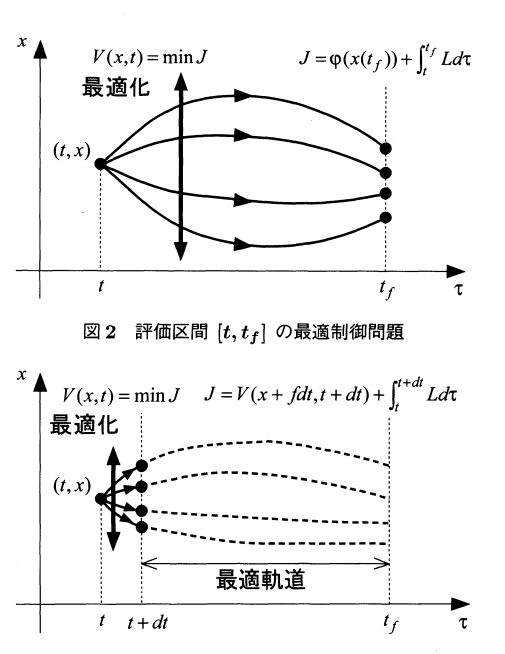
\includegraphics[clip, width = 4.0cm]{DP.png}
        \end{figure}
        \centering
        \tiny{
            \rightline{
                大塚:非線形最適制御入門
            }
        }
        動的計画法は大きな問題を小さな部分問題に分解し、それぞれ解くことで全体の解を得る手法
        \begin{itemize}
            \item 最適的な性質を持つ
            \item 計算結果を保存して再利用(メモ化)
        \end{itemize}
    \end{frame}
    
    \begin{frame}{動的計画法3}
        \scriptsize
        \fontsize{6.5pt}{6.5pt}\selectfont

        \begin{align*}
            V(x, t) &= \min_{u[t, t_f]} \left( \psi(x(t_f)) + \int_t^{t_f} L(x(\tau), u(\tau), \tau) d\tau \right) \\
            &= \min_{u[t, t_f]} \left( \int_t^{t+dt} L(x(\tau), u(\tau), \tau) d\tau + \colorbox{yellow}{$\psi(x(t_f)) + \int_{t+dt}^{t_f} L(x(\tau), u(\tau), \tau) d\tau$} \right) \\
            &= \min_{u[t, t+dt]} \left( \int_t^{t+dt} L(x(\tau), u(\tau), \tau) d\tau + \min_{u[t+dt, t_f]} \left( \psi(x(t_f)) + \int_{t+dt}^{t_f} L(x(\tau), u(\tau), \tau) d\tau \right) \right) \\
            &= \min_{u[t, t+dt]} \left( \int_t^{t+dt} L(x(\tau), u(\tau), \tau) d\tau + V \left( x + \int_t^{t+dt} f(x, u, \tau) d\tau, t + dt \right) \right) \\
        \end{align*}

        \begin{tcolorbox}[title=Bellman方程式]
            \begin{align*}
                &V(x, t) &=& \min_{u[t, t+dt]} \left( L(x, u, t) dt + V \left( x + f(x, u, t) dt, t + dt \right) \right) \\
                &V(x, t_f) &=& \psi(x(t_f))
            \end{align*}
        \end{tcolorbox}

        Bellman方程式が解ければ最適制御ができる!!!(もともとの評価関数を満たす解を求めるのと一緒) \\
        目標の状態$x(t_f)$が分かっていれば解けそう?? \\
    \end{frame}

    \begin{frame}{HJB方程式}
        \footnotesize
        \begin{tcolorbox}[title=Bellman方程式]
            \begin{align*}
                V(x, t) &= \min_{u[t, t+dt]} \left( L(x, u, t) dt + V \left( x + f(x, u, t) dt, t + dt \right) \right)
            \end{align*}
        \end{tcolorbox}
        \begin{tcolorbox}[title=次元の呪い]
            次元の呪いは、状態空間や行動空間の次元数が増加するにつれて、必要な計算量やメモリが指数的に増加する現象 \\
            2次元の格子が10の場合、合計100のセルが存在します。しかし、10次元の格子が各次元に10のセルを持つ場合、合計で$10^10 = 10,000,000,000$のセルが存在します。このように、次元が増加するにつれて格子の数が指数的に増加し、それに伴い計算量も指数的に増加します。
        \end{tcolorbox}
        次元の呪いのグラフを貼る \\
        \centering
    \end{frame}

    \begin{frame}{現在位置}
        \footnotesize
        \begin{itemize}
            \item 前回のおさらい
            \item 動的計画法
            \item \colorbox{yellow}{HJB方程式}
            \item 最小原理
            \item MPC導入
        \end{itemize}
        \begin{itembox}[l]{Bellman方程式からHJB方程式への変形}
            \begin{align*}
                V(x, t) &= \min_u \left( L(x, u, t) dt + V \left( x + f(x, u, t) dt, t + dt \right) \right)        
            \end{align*}
            \begin{align*}
                -\frac{\partial V}{\partial t}\left(x,t\right) = \min _u H\left(x, u, \left( \frac{\partial V}{\partial x} \right)^T\left(x, t\right), t \right)
            \end{align*}
        \end{itembox}
    \end{frame}

    \begin{frame}{HJB方程式}
        \fontsize{6.5pt}{6.5pt}\selectfont



        \colorbox{yellow}{$V(x, t) = \min_{u} \left( L(x, u, t) dt + V \left( x + f(x, u, t) dt, t + dt \right) \right)$} \\
        
        \begin{itembox}[l]{$V \left( x + f(x, u, t) dt, t + dt \right)$を$(x, t)$周りでTaylor展開をする}
            \begin{equation*}
                V \left( x + f(x, u, t) dt, t + dt \right) \simeq V \left(x, t\right) + \frac{\partial V}{\partial x}\left(x, t\right)f\left(x, u, t\right)dt + \frac{\partial V}{\partial t}\left(x, t\right)dt
            \end{equation*}
        \end{itembox}
        
        \begin{align*}
            V(x, t) &= \min_{u[t, t+dt]} \left( L(x, u, t) dt + V \left(x, t\right) + \frac{\partial V}{\partial x}\left(x, t\right)f\left(x, u, t\right)dt + \frac{\partial V}{\partial t}\left(x, t\right)dt \right) \\
            0&=\min_{u[t, t+dt]} \left( L(x, u, t) dt + \frac{\partial V}{\partial x}\left(x, t\right)f\left(x, u, t\right)dt + \frac{\partial V}{\partial t}\left(x, t\right)dt \right) \\
            H(x, u, \lambda, t) &= L(x, u, t) + \lambda^T f(x, u, t) \\
            H\left(x, u, \left( \frac{\partial V}{\partial x} \right)^T\left(x, t\right), t \right) &= L(x, u, t) + \frac{\partial V}{\partial x}\left(x, t\right)f\left(x, u, t\right) \\
        \end{align*}

        \colorbox{yellow}{$-\frac{\partial V}{\partial t}\left(x,t\right) = \min _u H\left(x, u, \left( \frac{\partial V}{\partial x} \right)^T\left(x, t\right), t \right)$} \\

    \end{frame}

    \begin{frame}{HJB方程式の解法}
        直接法\\
        間接法\\
        シューティング法とかの図をここに貼る \\
    \end{frame}

    \begin{frame}{現在位置}
        \footnotesize
        \begin{itemize}
            \item 前回のおさらい
            \item 動的計画法
            \item HJB方程式
            \item \colorbox{yellow}{最小原理}
            \item MPC導入
        \end{itemize}
        別の観点から最適制御を考える \\
        \begin{figure}[H]
            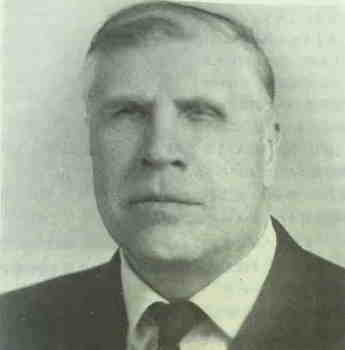
\includegraphics[clip, width = 2.0cm]{Pontryagin.png}
        \end{figure}
        \tiny{
            \rightline{
                Pontryagin
            }
        }
    \end{frame}

    \begin{frame}{最小原理1}
        \footnotesize

    \end{frame}

    \begin{frame}{最小原理2}
        \footnotesize
        もちろん最小原理からHJB方程式を導ける

    \end{frame}

    \begin{frame}{最適性条件まとめ}
        \footnotesize
        ラグランジュの未定乗数法\\
        KKT条件\\
        オイラーラグランジュ方程式\\
        動的計画法(new)\\
        HJB方程式(new)\\
        最小原理(new)\\
        動的計画法からHJB方程式を導いたが、最小原理からも導ける\\

        ここに各関係の図を貼る
    \end{frame}
    \begin{frame}{現在位置}
        \footnotesize
        \begin{itemize}
            \item 前回のおさらい
            \item 動的計画法
            \item HJB方程式
            \item 最小原理
            \item \colorbox{yellow}{MPC導入}
        \end{itemize}
    \end{frame}

    \begin{frame}{MPC}
        Euler-Lagrange方程式では入力に状態を含んでいないので、状態が変化(外的要因によって)する現実システムだと扱いにくい \\
        HJB方程式は入力に状態を含んでいるが、偏微分方程式なので扱いにくい \\
        現実問題に落とし込んだのがMPC \\
        評価区間が無限のMPCの解はHJB方程式と一致するはず(たぶん...) \\
    \end{frame}

    \begin{frame}{参考資料}
        \footnotesize

        書籍\\
        \begin{itemize}
            \item 非線形最適制御入門(名著です)
            \item しっかり学ぶ数理最適化(最適化全般について)
            \item はじめての最適化(変分法の説明が分かりやすいです)
        \end{itemize}
    \end{frame}
    
\end{document}